% !TEX root = main_jisa.tex
\documentclass[a4paper,fleqn]{cas-dc}

\usepackage[numbers,sort&compress]{natbib}
\usepackage{booktabs}
\usepackage{graphicx}
\usepackage{tabularx}
\usepackage{multirow}
\usepackage{amsmath}
\usepackage{xcolor}
\usepackage{url}

\newcommand{\dataset}[1]{\textsc{#1}}
\newcommand{\abbradv}{adversarial benign-prediction rate}
\newcommand{\silent}{residual silent-bypass rate}
\RenewDocumentCommand{\printorcid}{}{}

\begin{document}
\let\WriteBookmarks\relax
\def\floatpagepagefraction{0.8}
\def\textpagefraction{0.05}

\shorttitle{Evidence Boundaries of AST-Token-Only Defenses}
\shortauthors{K. Xie}

\title[mode=title]{Evidence Boundaries of AST-Token-Only Defenses against EaTVul-Style Insertion Evasion}

\author[1]{Kang Xie}
\cormark[1]
\ead{q1131714258@gmail.com}
\credit{Conceptualization, Methodology, Software, Validation, Formal analysis, Investigation, Data curation, Visualization, Writing -- original draft, Writing -- review and editing}

\affiliation[1]{organization={University of South China},
  city={Hengyang},
  postcode={421001},
  state={Hunan},
  country={China}}
\cortext[1]{Corresponding author}

\begin{abstract}
Insertion evasion can make a vulnerability detector accept still-vulnerable code. We ask what defensive action is justified when the available artifact contains only serialized AST-token sequences and detector outputs, but no authoritative source diff, insertion span, executable edit, control flow, or program dependence. We organize the study as an evidence boundary: observed evidence determines identifiable quantities; those quantities determine supported actions; stronger claims remain explicitly unsupported. A leakage-controlled protocol separates detector training, target-clean calibration, unattacked testing, and released adversarial testing, removes evaluation duplicates from all fitting roles under four content views, and evaluates a supervised gate and four anomaly detectors at 100 target--method--budget operating points. Screening behavior is strongly target dependent: at the nominal 5\% calibration budget, realized unattacked-review rates span 2.5--18.4\% and adversarial capture rates span 0--64\%, with method rankings changing across targets. A newly executed target-confidence control captures only 12 of 354 raw bypasses; removing 47 cross-dataset duplicate attack rows lowers its pooled capture among bypasses from 3.39\% to 2.82--3.11\%. A fixed exploratory grid of 972 token-deletion configurations yields zero median detector-output recovery in seven of eight target--diagnostic grids; the largest clean-utility-feasible reduction is 6\%. These results support target-specific quarantine only after local calibration and prospective load monitoring. They do not identify a corrected label, an inserted source region, or a safe automatic sanitization.
\end{abstract}

\begin{keywords}
software vulnerability detection \sep adversarial code \sep AST-token \sep quarantine \sep selective classification \sep anomaly detection
\end{keywords}

\maketitle

\section{Introduction}\label{sec:introduction}

Learning-based vulnerability detectors prioritize functions for security review, but their operational value depends on what happens to a benign prediction. A function predicted vulnerable usually enters an expensive analysis path; a function predicted benign may pass automatically. Insertion evasion exploits this asymmetry by retaining vulnerable behavior while adding code that moves the learned representation toward a benign decision. EaTVul demonstrates this threat against software vulnerability detectors using generated insertions and search over evasive variants \cite{liu2024eatvul}.

A response to suspicious input can take several forms. \emph{Screening} assigns a suspicion score. \emph{Quarantine} withholds a suspicious benign prediction from automatic acceptance and routes it to review. A \emph{diagnostic hard override} changes a benign prediction to vulnerable to measure an upper-bound intervention, with false alarms counted as classification errors. \emph{Diagnostic deletion} removes tokens and retests the target detector. Only a source-aware procedure that localizes the edit, preserves compilation, and validates security and functional behavior can support a claim of reliable automatic sanitization. We keep these actions distinct throughout the paper.

This distinction matters because the released artifact contains serialized AST-token sequences rather than authoritative source edits. It provides neither true insertion spans nor executable original/adversarial pairs. The central logic of this paper is therefore
\emph{observed evidence $\rightarrow$ identifiable quantities $\rightarrow$ supported action $\rightarrow$ unsupported claim}. Sample-level scores and disjoint clean calibration can identify review load and residual bypass on the fixed test rows; they can support quarantine. They cannot identify which source statements were inserted, whether deleting them preserves compilation and behavior, or whether a vulnerability has been removed.

We answer three research questions:
\begin{description}
\item[RQ1 (screening capability).] Under fixed per-target clean-calibration budgets, which silent-bypass and review-routing quantities can AST-token scores identify, and how much adversarial benign traffic do they capture?
\item[RQ2 (operational stability and transfer).] How stable are realized review load, capture, coverage, and method ranking across targets, budgets, and a bounded modern-target-model check?
\item[RQ3 (sanitization evidence).] Does a fixed exploratory token-deletion sensitivity grid provide evidence for reliable automatic sanitization, and which stronger quantities remain unidentifiable?
\end{description}

Our contributions are empirical and methodological rather than a claim of automatic repair. First, we define an evidence/action framework that separates sample-level screening, quarantine, hard override, diagnostic deletion, and source-aware sanitization. Second, we implement a leakage-controlled, matched-budget comparison of a supervised gate, Isolation Forest, One-Class SVM, Local Outlier Factor, and Mahalanobis distance on four EaTVul-style targets, retaining sample identifiers and four-view duplicate audits. Third, we quantify cross-target rank reversal, calibration-budget shift, and target heterogeneity instead of reporting a single favorable operating point. Fourth, we report a fixed 972-configuration deletion sensitivity study and state its causal limit: because the artifact cannot support a source-aware positive control, it cannot distinguish representation insufficiency from deletion-heuristic insufficiency.

\section{Background and related work}\label{sec:related}

\subsection{Vulnerability detection and dataset realism}

Neural vulnerability detectors range from sequence models such as VulDeePecker \cite{li2018vuldeepecker} to graph models such as Devign \cite{zhou2019devign} and transformer-based models such as LineVul \cite{fu2022linevul}. CodeBERT and GraphCodeBERT provide general code representations \cite{feng2020codebert,guo2021graphcodebert}. These advances do not remove evaluation risks: cross-dataset studies show that neural vulnerability detectors can be sensitive to dataset and feature choices \cite{chakraborty2020arewe}. Big-Vul links source changes with CVE metadata \cite{fan2020bigvul}; DiverseVul broadens project and weakness coverage \cite{chen2023diversevul}; and PrimeVul shows that duplicates, label quality, and unrealistic splits can materially distort code-language-model results \cite{ding2024primevul}. Our protocol therefore treats split identity and duplicate control as primary evidence rather than bookkeeping.

\subsection{Adversarial code and insertion evasion}

Semantics-preserving transformations can change predictions of code models \cite{yefet2020adversarial,ramakrishnan2020adversarial,rabin2020generalizability}, including optimized program obfuscations \cite{srikant2021optimized}. Natural Attack targets pretrained code models \cite{chen2022natural}; AdVulCode targets vulnerability detectors \cite{zhou2023advulcode}; and EaTVul uses generated insertions against software vulnerability detection \cite{liu2024eatvul}. CodeSearchAttack recently studies score-based black-box attacks over code substitutions in JISA \cite{pu2025codesearchattack}. These attacks differ in transformation, target access, and validation. We do not regenerate attacks or claim semantic preservation beyond the provenance of the released EaTVul-style samples; we evaluate defensive decisions on those fixed artifacts.

\subsection{Detection, abstention, and validated repair}

Adversarial-example and out-of-distribution detection provide alarms rather than corrected ground truth \cite{biggio2018wild,nist2024aml}. Classification with a reject option instead frames abstention through risk and coverage \cite{chow1970reject,geifman2017selective,geifman2019selectivenet}; Deep Gamblers provides a complementary learned-abstention formulation \cite{liu2019deepgamblers}. This view motivates quarantine as a measurable routing policy. By contrast, source-aware localization and repair require program structure and validation. Program slicing and dependence graphs provide source-level analysis objects \cite{weiser1984program,ferrante1987pdg}; APR4Vul shows that even patches passing end-to-end tests can remain security- or functionality-incorrect \cite{bui2024apr4vul}. Token deletion followed only by a model query is therefore a diagnostic, not repair validation.

\begin{table*}[t]
\centering
\caption{Closest-work comparison. ``C/S validation'' denotes compilation plus security/functional validation. A dash means the work does not perform a defense action of that type.}
\label{tab:closest}
\scriptsize
\resizebox{\textwidth}{!}{%
\begin{tabular}{lllllllllll}
\toprule
Work & Attack & Input & Target & Action & Spans & CFG/PDG & Quarantine & Localization & C/S validation & Difference here \\
\midrule
LineVul \cite{fu2022linevul} & -- & source lines & Transformer & detect vuln. & line labels & no & no & yes & no & defense after evasion \\
Natural Attack \cite{chen2022natural} & renaming & source tokens & code PTMs & attack & identifiers & no & no & changed vars & execution checks & insertion defense \\
AdVulCode \cite{zhou2023advulcode} & code transform & source code & vuln. detectors & attack & edit sites & no & no & attack edits & syntax/semantics & artifact-only response \\
EaTVul \cite{liu2024eatvul} & insertion & source/AST artifact & vuln. detectors & attack & attack process & model dependent & no & attack edits & attack validation & evaluates defenses \\
CodeSearchAttack \cite{pu2025codesearchattack} & substitution & source code & code models & attack & variables & no & no & changed vars & executability goal & insertion and quarantine \\
PrimeVul \cite{ding2024primevul} & -- & source functions & code LMs & dataset/eval. & paired funcs. & no & no & no & label audit & adversarial routing \\
APR4Vul \cite{bui2024apr4vul} & -- & executable source & repair tools & repair & source faults & tool dependent & no & supplied/evaluated & yes & no repair claim \\
This work & insertion & serialized AST-token & LR + CodeBERT & screen/route & unavailable & unavailable & yes & diagnostic only & unavailable & evidence/action boundary \\
\bottomrule
\end{tabular}}
\end{table*}

\section{Evidence, threat, and action boundary}\label{sec:model}

The defender receives a serialized AST-token sequence $x$, a target prediction $\hat y\in\{0,1\}$, and optionally a vulnerable-class probability. It does not receive an authoritative source diff, exact insertion boundary, parser-reconstructable tree, CFG, PDG, executable edit, or complete original-to-attack identifier. The attacker is represented by the released adversarial test rows: every row is labeled vulnerable, while a silent bypass is a row for which the target detector predicts benign. Because complete pairing is absent, we call the measured fraction the \abbradv, not conventional attack success rate.

The screening method produces $s(x)\in\mathbb{R}$. Let $C_0$ be target-clean calibration rows that are truly benign and predicted benign. For nominal budget $b$, the threshold is the empirical $(1-b)$ quantile $t_b=Q_{1-b}(\{s(x):x\in C_0\})$. A test row is reviewed exactly when $q_b(x)=\mathbf{1}[\hat y=0\wedge s(x)\ge t_b]$; quarantine does not change $\hat y$. For an adversarial set $A$ and clean test set $T$, capture is $|A|^{-1}\sum_{x\in A}\mathbf{1}[\hat y=0]q_b(x)$, residual silent bypass is $|A|^{-1}\sum_{x\in A}\mathbf{1}[\hat y=0](1-q_b(x))$, and clean review is $|T|^{-1}\sum_{x\in T}q_b(x)$. Conditional clean review uses predicted-benign clean rows as denominator. Coverage is the fraction of clean rows auto-passed after original vulnerable predictions and quarantined benign predictions are withheld.

We use five evidence levels to prevent an action from outrunning its observations. Level~1 is the AST-token sequence and target output. Level~2 adds disjoint roles, identifiers, hashes, and target-clean calibration. Level~3 adds sample-level screening outcomes, which identify review, capture, residual bypass, coverage, and selective risk on the fixed samples. Level~4 would require authoritative paired source and inserted spans. Level~5 would additionally require compilable edits plus security and functional validation. This study reaches Levels~1--3. Quarantine is supported there; label correction, source localization, and reliable automatic sanitization require evidence at Levels~4--5.

Figure~\ref{fig:boundary} summarizes this boundary. Diagnostic hard override changes labels and therefore incurs classification errors. Diagnostic deletion observes only whether the target output changes after serialized-token removal. Neither action supplies the missing source-aware evidence.

\begin{figure*}[t]
\centering
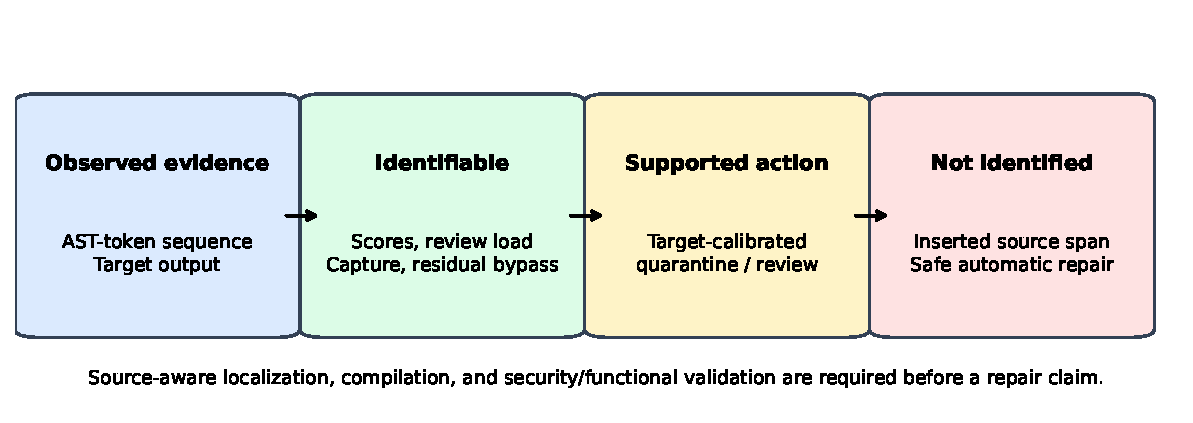
\includegraphics[width=0.92\textwidth]{../figures_submission_jisa/action_boundary.pdf}
\caption{Observation/action boundary. Serialized AST-token sequences and target outputs support sample-level screening and review routing. Hard override and token deletion remain diagnostics. A reliable automatic-sanitization claim additionally requires source-aware localization, compilation, and semantic validation.}
\label{fig:boundary}
\end{figure*}

\section{Methods mapped to the research questions}\label{sec:methods}

\subsection{Target detectors}

\begingroup\sloppy
The auditable baseline is a TF--IDF logistic-regression detector fitted on each target's detector-training role. RQ2 also includes a bounded CodeBERT target check on two outer targets. Its checkpoint is \texttt{microsoft/\allowbreak codebert-base}; the pinned revision is \texttt{3b0952fe\allowbreak ddeffad0\allowbreak 063f2740\allowbreak 80e3c23d\allowbreak 75e7eb39}. The 498,627,950-byte weight file has SHA-256 \texttt{28b61fd8\allowbreak fa069f6b\allowbreak c966f4cb\allowbreak 9572a402\allowbreak 6ab2a784\allowbreak fca8fb22\allowbreak 4020d91b\allowbreak 744e32d6}. After deterministic class-capped sampling from detector training, a stratified 20\% internal model-validation fold selects among at most three class-weighted fine-tuning epochs by validation F1, then validation loss, then the earliest epoch. The base checkpoint is reinitialized and trained for the selected epoch count on the internal-training partition. Target-clean calibration, clean test, and adversarial test are not queried during checkpoint selection; calibration and both evaluation roles are queried only after the final retraining. All steps use seed 7, maximum length 256, batch size 4, and learning rate $2\times10^{-5}$. This is a CodeBERT-based vulnerability classifier, not LineVul: the official LineVul interface expects source-text functions, whereas the released inputs are serialized AST-token sequences.
\par\endgroup

\subsection{Supervised gate and anomaly baselines}

For RQ1, the supervised gate is trained on filtered clean and adversarial source roles from non-target datasets. Its features combine TF--IDF and structural summary statistics. The four anomaly baselines fit only the target detector-training role and receive no attack labels: Isolation Forest, One-Class SVM, Local Outlier Factor, and Mahalanobis distance after the same TF--IDF/SVD and structural transformation. Every method returns a continuous score.

For each method and target, thresholds are selected independently at nominal review budgets of 1\%, 3\%, 5\%, 10\%, and 15\%. The main screening grid retains the original inclusive empirical-quantile rule. Consequently, its realized rate can differ because of both threshold ties and calibration-to-test shift. RQ2 reports (i) realized-rate ranges and maximum absolute budget deviation at nominal 5\%, (ii) target-local method ranks ordered by higher capture, smaller absolute review deviation, and method name, and (iii) the fixed-grid point closest to 5\% realized review for each target--method pair. A separate target-confidence control uses a deterministic hash-based exact-$k$ tie policy, so its calibration rounding/tie effect and calibration-to-test drift are reported separately. The closest-rate quantity is a post hoc stability description, not a deployment-selection rule.

\subsection{Diagnostic deletion for RQ3}

The fixed-window diagnostic tests window sizes 128, 256, 512, 1024, and 1536 tokens; stride ratios 0.25, 0.50, and 0.75; clean-utility budgets 0.01, 0.03, and 0.05; and vulnerable-probability gains 0, 0.001, and 0.005. This yields 135 configurations per target. The approximate AST-token-component diagnostic tests maximum cluster sizes 1, 2, 3, and 5; one to three selected spans; the same three clean-utility budgets; and the same three gains, yielding 108 configurations per target. In total, 243 configurations are evaluated on each of four targets.

For every configuration we retain sample-level before/after predictions, modification indicators, and removed-token ratios. We report adversarial and clean modification rates, removed-token mean/median/IQR, detector-output recovery, and clean F1 change. Removed-token ratios are not insertion recall. The deletion grid is a fixed exploratory sensitivity analysis rather than a model-selection procedure. No configuration selected from the adversarial test grid is presented as a deployable sanitizer. ``Best feasible'' denotes only the largest observed detector-output reduction among fixed grid cells whose clean-F1 drop is at most 0.03; it is an exploratory upper bound, not a selected operating point.

\section{Leakage-controlled experimental protocol}\label{sec:protocol}

\subsection{Roles and duplicate control}

For every outer target, the source training split is deterministically divided into disjoint detector-training and target-clean calibration roles with seed 7. Final metrics are computed once on the untouched target-clean test and target-adversarial test roles. Gate fitting uses filtered non-target source roles. Target adversarial rows are never used for fitting, model selection, threshold selection, or calibration. Sample identifiers and role hashes are persisted before fitting, and every paper-facing row is traceable to a run manifest and sample-level log.

The audit computes SHA-256 over raw text, normalized comments and whitespace, serialized tokens, and normalized identifiers. Every evaluation row remains fixed. Any matching row is removed from fitting, validation, and calibration pools, and the removal registry and role digests are persisted. The audit confirms 47 serialized-token duplicates between the \dataset{ASTERISK} and \dataset{OPENSSL} adversarial splits. The available \texttt{project} field behaves as a per-function row identifier rather than authoritative repository provenance; consequently, source-project overlap and project-coherent explanations are not claimed.

\IfFileExists{generated/jisa_dataset_profile.tex}{\begin{table*}[t]
\centering
\caption{Dataset roles and median serialized AST-token lengths. ADV denotes the released adversarial test role.}
\label{tab:dataset-profile}
\scriptsize
\begin{tabular}{lrrrrrr}
\toprule
Target & Train & Test & ADV & Train med. & Test med. & ADV med. \\ 
\midrule
ASTERISK & 880 & 367 & 50 & 4277 & 3893 & 4697 \\
OPENSSL & 520 & 213 & 50 & 1449 & 1546 & 4697 \\
CWE119 & 5670 & 2451 & 200 & 2151 & 2044 & 1800 \\
CWE399 & 545 & 255 & 200 & 2547 & 2356 & 2192 \\
\bottomrule
\end{tabular}
\end{table*}
}{}

\subsection{Metrics and uncertainty}

For each target, method, and budget we report raw adversarial benign predictions; captured and residual counts; unattacked and conditional review rates; coverage; selective risk among auto-passed unattacked rows; and baseline unattacked F1. We omit ``number needed to review'' because it mixes unattacked and adversarial rows and therefore changes with the artificial attack prevalence in the evaluation stream. Wilson 95\% intervals are reported for binomial rates. Before/after diagnostic decisions use paired bootstrap intervals with fixed seeds. The budget grid is descriptive, no favorable cell is promoted as confirmatory, and no claim is selected from multiple McNemar tests. Macro summaries weight targets equally; micro summaries are accompanied by cross-dataset duplicate sensitivity because target sizes and duplicate counts differ substantially.

RQ1 is answered by the fixed matched-budget counts and rates. RQ2 is answered by target-wise ranges, ordinal rank spans, closest-realized-rate summaries, coverage curves, and the bounded CodeBERT check; with four targets, target characteristics are shown only as context and no correlation is estimated. RQ3 is answered by medians, IQRs, maxima, and clean-utility-feasible maxima over the entire fixed deletion grid. The absence of source spans makes localization precision, insertion recall, compilation success, and semantic repair success non-identifiable.

\section{Results by research question}\label{sec:results}

\subsection{RQ1: screening capability and identifiable routing quantities}

The raw target detectors produce 32/50, 38/50, 144/200, and 140/200 adversarial benign predictions on \dataset{ASTERISK}, \dataset{OPENSSL}, \dataset{CWE119}, and \dataset{CWE399}, respectively. The evaluation then fixes 100 operating points: four targets, five screening families, and five calibration budgets. Table~\ref{tab:matched-five} gives the nominal 5\% slice using only the quantities needed for the main operational comparison; conditional review, selective risk, capture precision, all budgets, and Wilson intervals remain in the supplement.

At this slice, the supervised gate captures 1, 5, 7, and 32 adversarial benign predictions, but its realized clean-review rate ranges from 0.035 to 0.149. Generic anomaly detectors exceed the gate on selected targets: on \dataset{OPENSSL}, they capture 19--32 outcomes at realized clean-review rates of 0.033--0.070, versus 5 at 0.070 for the gate. On \dataset{ASTERISK}, every method captures at most two. These counts identify which fixed samples would be withheld and the associated clean review load; they do not identify corrected labels.

\IfFileExists{generated/jisa_matched_budget_5.tex}{\begin{table*}[t]
\centering
\caption{Matched screening at the nominal 5\% calibration budget. Counts are shown to avoid prevalence-dependent composites.}
\label{tab:matched-five}
\scriptsize
\begin{tabular}{llrrr}
\toprule
Target & Method & Unattacked review & Captured/bypass & Residual/all ADV \\ 
\midrule
ASTERISK & Supervised Gate & 19/367 (5.2\%) & 1/32 & 31/50 \\
ASTERISK & Isolation Forest & 24/367 (6.5\%) & 2/32 & 30/50 \\
ASTERISK & One-Class SVM & 21/367 (5.7\%) & 0/32 & 32/50 \\
ASTERISK & Local Outlier Factor & 9/367 (2.5\%) & 1/32 & 31/50 \\
ASTERISK & Mahalanobis & 19/367 (5.2\%) & 2/32 & 30/50 \\
OPENSSL & Supervised Gate & 15/213 (7.0\%) & 5/38 & 33/50 \\
OPENSSL & Isolation Forest & 11/213 (5.2\%) & 23/38 & 15/50 \\
OPENSSL & One-Class SVM & 15/213 (7.0\%) & 32/38 & 6/50 \\
OPENSSL & Local Outlier Factor & 7/213 (3.3\%) & 19/38 & 19/50 \\
OPENSSL & Mahalanobis & 11/213 (5.2\%) & 26/38 & 12/50 \\
CWE119 & Supervised Gate & 85/2451 (3.5\%) & 7/144 & 137/200 \\
CWE119 & Isolation Forest & 129/2451 (5.3\%) & 12/144 & 132/200 \\
CWE119 & One-Class SVM & 131/2451 (5.3\%) & 11/144 & 133/200 \\
CWE119 & Local Outlier Factor & 84/2451 (3.4\%) & 0/144 & 144/200 \\
CWE119 & Mahalanobis & 136/2451 (5.5\%) & 13/144 & 131/200 \\
CWE399 & Supervised Gate & 38/255 (14.9\%) & 32/140 & 108/200 \\
CWE399 & Isolation Forest & 38/255 (14.9\%) & 40/140 & 100/200 \\
CWE399 & One-Class SVM & 47/255 (18.4\%) & 42/140 & 98/200 \\
CWE399 & Local Outlier Factor & 25/255 (9.8\%) & 24/140 & 116/200 \\
CWE399 & Mahalanobis & 32/255 (12.5\%) & 32/140 & 108/200 \\
\bottomrule
\end{tabular}
\end{table*}
}{}

\paragraph{Target-confidence control and tie decomposition.}
As a prevalence-independent selective-classification baseline, we retrained the TF--IDF logistic-regression target model for each dataset on a stratified 80\% detector-training role and calibrated vulnerable-class probability on the remaining 20\% (seed 7). Only true-benign, predicted-benign calibration rows determine the review threshold; the official unattacked and adversarial test roles are queried after calibration. The deterministic exact-$k$ policy breaks a boundary tie by a SHA-256 ordering of sample identifiers. Table~\ref{tab:confidence-baseline} shows that the 5\% control captures only 2, 3, 6, and 1 raw bypasses, respectively. Its boundary scores have no ties at this operating point; the remaining 0.4--3.8 percentage-point mismatch is calibration-to-test drift rather than quantile tie overshoot. This weak control rules out the simple explanation that target uncertainty alone accounts for the stronger target-specific anomaly results.

\begin{table}[t]
\centering
\caption{Target-confidence baseline at a 5\% nominal calibration budget. Review and capture are evaluated on untouched test roles.}
\label{tab:confidence-baseline}
\scriptsize
\begin{tabular}{lrrrrrr}
\toprule
Target & Cal. $n$ & Tie over. & Drift & Review & Captured & Residual \\
\midrule
ASTERISK & 151 & 0.0 pp & 0.4 pp & 5.4\% & 2/32 & 60.0\% \\
OPENSSL & 77 & 0.0 pp & 2.6 pp & 6.1\% & 3/38 & 70.0\% \\
CWE119 & 666 & 0.0 pp & 1.3 pp & 4.3\% & 6/144 & 69.0\% \\
CWE399 & 61 & 0.0 pp & 3.8 pp & 6.3\% & 1/140 & 69.5\% \\
\bottomrule
\end{tabular}
\end{table}


The 47 serialized-token duplicates shared by the \dataset{ASTERISK} and \dataset{OPENSSL} adversarial roles affect pooled summaries even though target-wise rows remain fixed. Deterministically retaining the first occurrence in forward and reverse target order gives a sensitivity interval rather than privileging one target model. At 5\%, pooled confidence-baseline capture among raw bypasses falls from 3.39\% to 2.82--3.11\% (Table~\ref{tab:duplicate-sensitivity}). We therefore use target-wise or macro summaries for claims and treat pooled micro values as duplicate-sensitive.

\begin{table}[t]
\centering
\caption{Micro-average duplicate sensitivity for the confidence baseline at 5\%.}
\label{tab:duplicate-sensitivity}
\scriptsize
\begin{tabular}{lrrrr}
\toprule
Analysis & Rows & Unique & Captured & Capture/bypass \\
\midrule
all rows & 500 & 453 & 12 & 3.4\% \\
deduplicated forward & 453 & 453 & 9 & 2.8\% \\
deduplicated reverse & 453 & 453 & 10 & 3.1\% \\
\bottomrule
\end{tabular}
\end{table}


\paragraph{Answer to RQ1.} AST-token scores identify sample-level capture, residual bypass, review load, coverage, and selective risk on the fixed test roles. They can support calibrated quarantine. Screening capability is target dependent, and the evidence does not support label correction or a universally dominant screening family.

\subsection{RQ2: operational stability, budget transfer, and model scope}

Figure~\ref{fig:capture} plots capture against realized clean-review rate across all budgets. Figure~\ref{fig:coverage} plots residual silent bypass against clean coverage. The curves expose the operational choice hidden by a nominal threshold: gains on \dataset{OPENSSL} are achievable at modest review load, whereas the same method/rate relationship does not transfer uniformly.

\begin{figure*}[t]
\centering
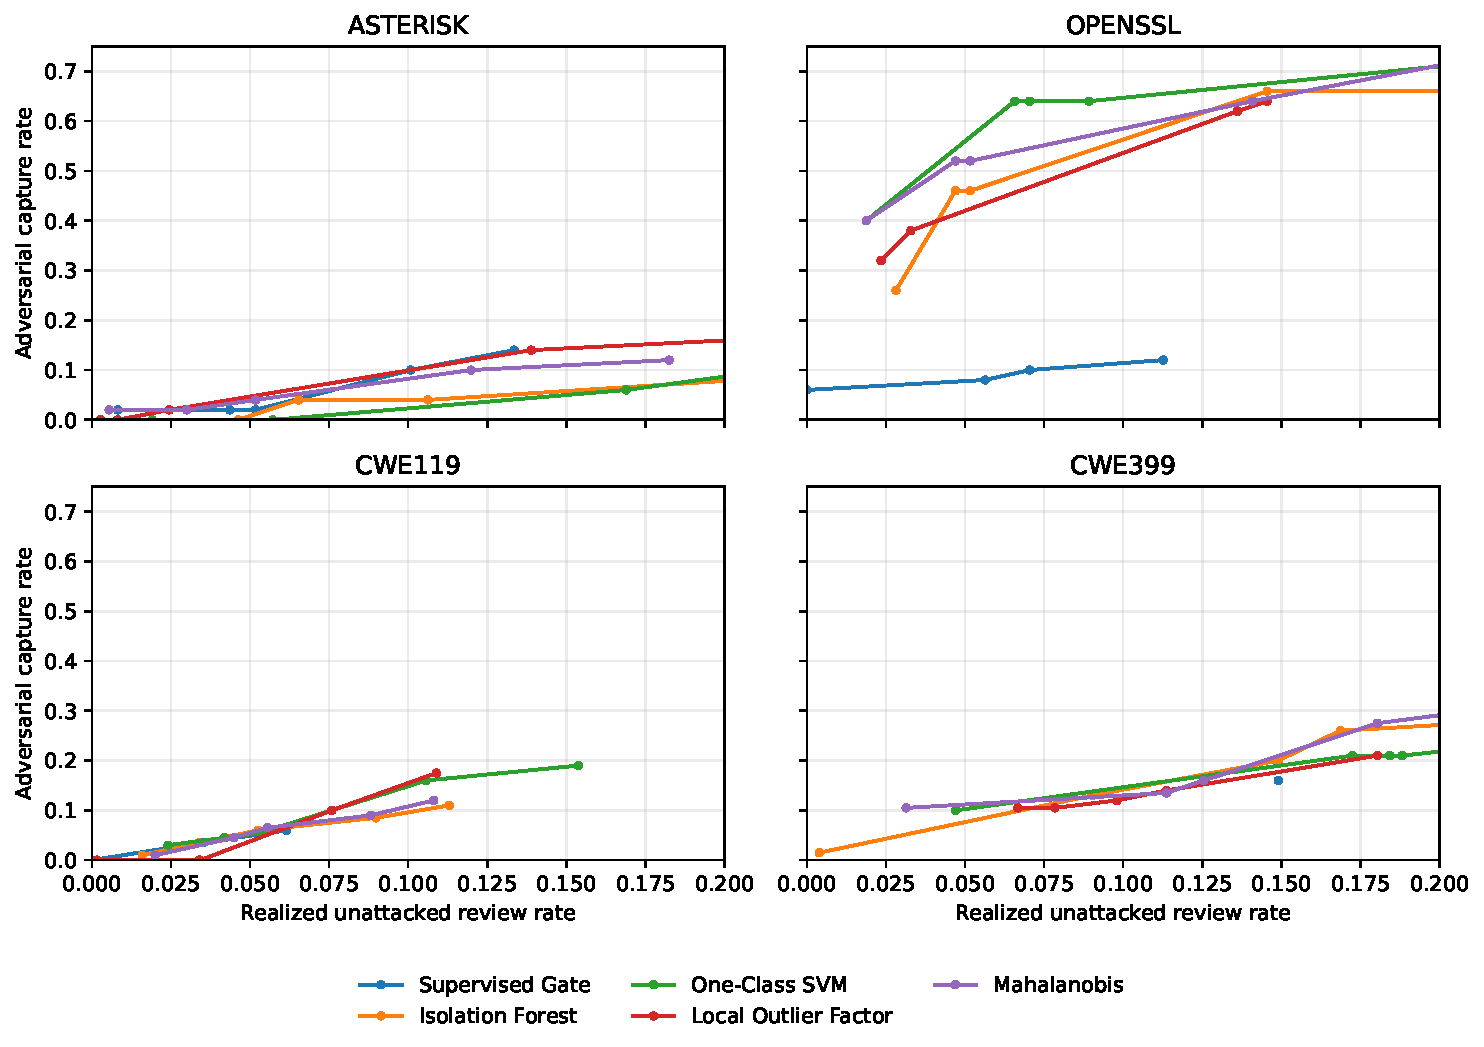
\includegraphics[width=0.92\textwidth]{../figures_submission_jisa/capture_vs_review.pdf}
\caption{Adversarial capture rate versus realized unattacked-review rate. All panels share both axes. Each line uses the same nominal budget grid, but the horizontal coordinate is the observed target-test rate. Target-dependent slopes and crossings preclude a common method ranking.}
\label{fig:capture}
\end{figure*}

\begin{figure*}[t]
\centering
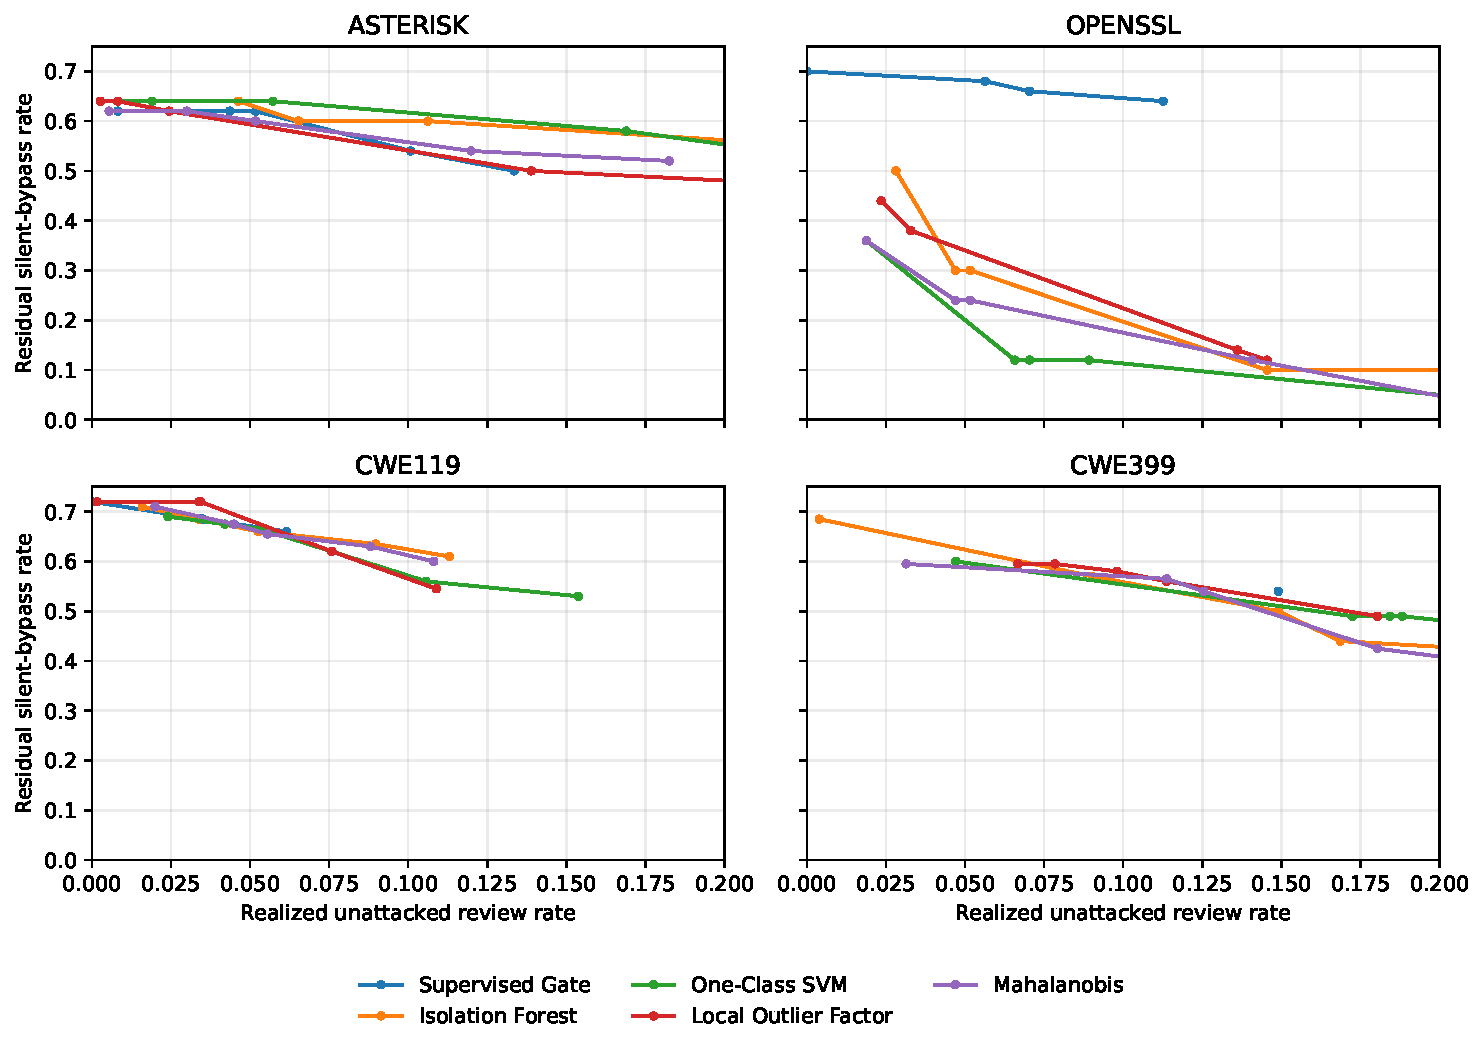
\includegraphics[width=0.92\textwidth]{../figures_submission_jisa/residual_vs_review.pdf}
\caption{Residual silent-bypass rate versus realized unattacked-review rate. All panels share both axes. Lower residual bypass and lower review load are preferred; no screening family occupies that region uniformly across the four targets.}
\label{fig:coverage}
\end{figure*}

Table~\ref{tab:screening-stability} quantifies this variation at the nominal 5\% budget. Realized review spans 0.025--0.184 across all target--method pairs, and the largest within-method deviation from 0.05 is 0.134. One-Class SVM has target-local ranks from first to fifth; Mahalanobis ranks first on two targets but only third on another. The closest-realized-rate and target-context tables in the supplement show that calibration budget is not portable: for the supervised gate, the closest fixed-grid point to 0.05 uses nominal 0.15 on \dataset{CWE119}, yet nominal 0.01 on \dataset{CWE399} still realizes 0.149 review. With only four targets, the accompanying token-length and vocabulary profiles are descriptive; no correlation is claimed.

\IfFileExists{generated/jisa_screening_stability.tex}{\begin{table}[t]
\centering
\caption{Cross-target operating stability at the nominal 5\% budget.}
\label{tab:screening-stability}
\scriptsize
\begin{tabular}{lrrr}
\toprule
Method & Realized review range & Max. deviation & Rank span \\ 
\midrule
Supervised Gate & 3.5--14.9\% & 9.9 pp & 3--5 \\
Isolation Forest & 5.2--14.9\% & 9.9 pp & 2--3 \\
One-Class SVM & 5.3--18.4\% & 13.4 pp & 1--5 \\
Local Outlier Factor & 2.5--9.8\% & 4.8 pp & 4--5 \\
Mahalanobis & 5.2--12.5\% & 7.5 pp & 1--3 \\
\bottomrule
\end{tabular}
\end{table}
}{}

\paragraph{Bounded modern target-model check.}

\IfFileExists{generated/jisa_codebert_results.tex}{\begin{table}[t]
\centering
\caption{Bounded CodeBERT feasibility check. The 256-token prefix truncates most serialized inputs; these rows are not main efficacy evidence.}
\label{tab:codebert-results}
\scriptsize
\begin{tabular}{lrrrrrr}
\toprule
Target & Epoch & Precision & Recall & F1 & Raw bypass & Residual \\ 
\midrule
ASTERISK & 2 & 0.150 & 1.000 & 0.261 & 0.480 & 0.440 \\
OPENSSL & 3 & 0.298 & 0.973 & 0.456 & 0.340 & 0.320 \\
\bottomrule
\end{tabular}
\end{table}
}{}
The CodeBERT experiment is a bounded transfer check on two targets rather than evidence of universal model-family generalization. More fundamentally, its 256-token prefix is much shorter than the serialized inputs: 84--100\% of official unattacked test rows and 90--100\% of adversarial rows exceed 256 tokens (Table~\ref{tab:length-truncation}). Internal validation selects epoch 2 on \dataset{ASTERISK} and epoch 3 on \dataset{OPENSSL}. Unattacked-test precision/recall/F1 are 0.150/1.000/0.261 and 0.298/0.973/0.456, respectively; the corresponding validation F1 values are 0.917 and 0.824. This validation-to-test gap and severe prefix truncation make the rows a provenance/feasibility check, not comparative efficacy evidence. On \dataset{ASTERISK}, the gate captures 2 of 24 adversarial benign outcomes; on \dataset{OPENSSL}, it captures 1 of 17. A defensible modern-model extension requires chunked long-sequence aggregation or a source-text model evaluated on inputs matching its training domain.

\begin{table}[t]
\centering
\caption{Serialized AST-token length relative to the 256-token CodeBERT limit.}
\label{tab:length-truncation}
\scriptsize
\begin{tabular}{llrrr}
\toprule
Target & Role & Median & P95 & $>256$ \\
\midrule
ASTERISK & test & 3893 & 15188 & 83.9\% \\
ASTERISK & adv & 4698 & 12694 & 90.0\% \\
OPENSSL & test & 1546 & 11444 & 88.3\% \\
OPENSSL & adv & 4698 & 12877 & 90.0\% \\
CWE119 & test & 2044 & 4540 & 100.0\% \\
CWE119 & adv & 1800 & 4497 & 100.0\% \\
CWE399 & test & 2356 & 6064 & 100.0\% \\
CWE399 & adv & 2192 & 5335 & 100.0\% \\
\bottomrule
\end{tabular}
\end{table}


\paragraph{Answer to RQ2.} Operational behavior is not stable across targets. Realized budget, capture, coverage, and method ordering all shift, and the bounded CodeBERT check does not establish broad model-family transfer. Deployment therefore requires target-specific calibration, prospective monitoring, and an explicit review-capacity policy.

\subsection{RQ3: evidence from diagnostic deletion}

Seven of eight target--deletion-family grids have zero median adversarial benign-prediction-rate reduction; the \dataset{OPENSSL} component grid has median 0.010. Under a maximum clean-F1 drop of 0.03, the largest observed feasible reduction is 0.015 for fixed-window deletion on \dataset{CWE119} and 0.060 on \dataset{OPENSSL}; it is zero on \dataset{ASTERISK} and \dataset{CWE399}. Approximate component deletion reaches at most 0.005 on \dataset{CWE119} and 0.040 on \dataset{OPENSSL}, with zero feasible maximum on \dataset{CWE399}; no \dataset{ASTERISK} component configuration satisfies the clean-utility limit. These maxima are exploratory upper bounds from the fixed adversarial grid. They do not establish a stable or deployable sanitizer.

\IfFileExists{generated/jisa_deletion_sensitivity.tex}{\begin{table*}[t]
\centering
\caption{Full fixed deletion grid. Best feasible is the largest reduction with clean-F1 drop at most 0.03 and is exploratory, not selected for deployment.}
\label{tab:deletion-sensitivity}
\scriptsize
\begin{tabular}{llrrrr}
\toprule
Target & Diagnostic & Cells & Median & IQR & Best feasible \\ 
\midrule
ASTERISK & localize & 135 & 0.0\% & 0.0--0.0\% & -- \\
ASTERISK & component & 108 & 0.0\% & 0.0--0.0\% & -- \\
OPENSSL & localize & 135 & 0.0\% & 0.0--2.0\% & 6.0\% \\
OPENSSL & component & 108 & 1.0\% & 0.0--4.0\% & 4.0\% \\
CWE119 & localize & 135 & 0.0\% & 0.0--0.0\% & 1.5\% \\
CWE119 & component & 108 & 0.0\% & 0.0--0.0\% & 0.5\% \\
CWE399 & localize & 135 & 0.0\% & 0.0--0.0\% & 0.0\% \\
CWE399 & component & 108 & 0.0\% & 0.0--0.0\% & 0.0\% \\
\bottomrule
\end{tabular}
\end{table*}
}{}

The evaluated fixed-window and approximate AST-token-component deletion methods did not provide reliable detector-output recovery under the tested configurations. More importantly, the dataset does not provide insertion-span ground truth, authoritative source pairs, or executable edits. A source-aware positive control---for example, removing a known inserted source span and then compiling and validating the result---cannot be constructed from the available files. The experiment therefore cannot distinguish an insufficient AST-token representation from insufficient deletion heuristics, and localization precision/recall, compilation success, and paired repair success are not identifiable.

\paragraph{Answer to RQ3.} The fixed deletion grid provides negative sensitivity evidence about the tested token-removal procedures and target outputs only. It provides no evidence of reliable automatic sanitization and cannot isolate why recovery is weak without a source-aware positive control.

\section{Discussion: supported actions and unsupported claims}\label{sec:deployment}

The evidence chain yields one conditionally supported operational action. Disjoint unattacked calibration and sample-level scores identify review load, captured adversarial benign predictions, residual bypass, and coverage on the fixed roles. Those quantities can support target-specific quarantine only after local validation: withhold selected benign predictions and route them to a stronger analyzer or human reviewer. A prospective deployment must state review capacity, calibrate on local unattacked traffic, monitor realized rather than nominal review, and predefine the downstream process. Weak \dataset{ASTERISK} results and the confidence-control failure preclude a general deployment recommendation.

Three stronger claims remain unsupported. First, diagnostic hard override does not establish the corrected label and can lower clean F1. Second, a target-output change after token deletion does not identify an inserted source region. Third, no result establishes that an edit compiles, removes a vulnerability, preserves functionality, or avoids semantic side effects. A production sanitizer would need an authoritative source diff or source-aware localization, parser-valid edits, compilation, vulnerability-specific tests or static/dynamic analysis, regression tests, and review of side effects.

The target heterogeneity also argues against deploying one threshold or screening family unchanged across projects. The \dataset{OPENSSL} anomaly results do not establish general anomaly-detector superiority, and the stronger \dataset{CWE399} gate result does not establish supervised-gate superiority. These are observed target-specific rankings, not a universal method comparison.

\section{Threats to validity}\label{sec:threats}

\textbf{Construct validity.} The adversarial benign-prediction rate uses all released adversarial rows because complete original-to-attack pairing is unavailable; it is not conventional attack success rate. Quarantine review rates measure routing, not corrected labels. Deletion recovery measures target-output changes, not insertion removal. Without true source spans and an executable positive control, the study cannot distinguish representation insufficiency from deletion-heuristic insufficiency.

\textbf{Internal validity.} Target-clean calibration is disjoint from target-clean test, and target adversarial tests are excluded from fitting, checkpoint selection, and threshold selection. Four hash views reduce exact and normalized content leakage. They cannot detect semantically equivalent code with unrelated serialization, and unavailable source-project metadata prevents repository-level overlap claims. The closest-realized-rate table is computed after evaluation only to describe budget shift and is not used to choose a reported deployable configuration.

\textbf{External validity.} The main evidence covers four fixed AST-token datasets and an auditable logistic-regression target; the modern-model check covers only two targets with a CodeBERT-based classifier whose 256-token prefix truncates most inputs. It is not a LineVul replication and does not establish transfer to graph models, repository-level scanners, other attacks, other serializations, or prospective project traffic. Four targets are insufficient for a defensible correlation between corpus characteristics and defense outcomes.

\textbf{Statistical conclusion validity.} Wilson intervals describe uncertainty for fixed released samples, and paired bootstrap describes decision sensitivity on those samples; neither is an independent replication from a population of generated attacks. Targets differ greatly in size, so both target-level and macro/micro summaries are required. Ordinal rank spans are descriptive and unstable under ties. The deletion grid is exploratory, and its maxima are reported alongside medians and IQRs rather than treated as selected estimates.

\textbf{Artifact validity.} The received files omit authoritative repository provenance, complete original/adversarial identifiers, inserted spans, parser-reconstructable trees, and executable source. Raw AST-token splits are not redistributed because authorization is not established. Hash-bound derived logs make the reported computations auditable, but they cannot recreate missing semantic evidence or independently verify the attack-generation process.

\section{Reproducibility and artifact availability}\label{sec:artifact}

The submission artifact contains three clearly separated categories. First, redistributable derived material includes role identifiers and hashes, duplicate-removal registries, per-sample decisions without raw function text, aggregate CSVs, configurations, vector figures, and verification scripts. Every paper-facing run manifest records commands, inputs, outputs, package versions, timestamps, and SHA-256 digests. Second, the received AST-token split files are required local inputs but are not included in public Git tracking because redistribution authorization is not established. Third, authoritative source diffs, insertion spans, executable paired edits, and complete original/adversarial identifiers were not present and cannot be reconstructed from the derived artifact.

The primary tables can be rebuilt from the documented local inputs; the verifier recomputes the new confidence-control summaries from 2,500 adversarial target--budget rows and checks SHA-256 digests before table generation. The verified legacy evidence bundle contains the fixed-grid summaries and hashes of the larger archived outputs. The runbook gives preparation paths, checksums, and expected counts for non-redistributed inputs. No public release tag or archival DOI is claimed; before submission, the derived artifact must either be deposited and cited with a persistent identifier or the submission system must carry the same explicit access limitation.

The nested leave-one-dataset-out hard-override analysis is retained in the supplement as a robustness diagnostic. Its protocol was frozen before the final evaluation at the artifact revision recorded in the evidence manifest; it did not meet its frozen macro-reduction and universal clean-utility criteria and is not promoted over the matched-budget quarantine evidence.

\section{Conclusion}\label{sec:conclusion}

This study connects evidence to identifiable quantities and then to defensible action. Under leakage-controlled, matched-budget evaluation, AST-token scores identify target-specific review, capture, residual-bypass, coverage, and selective-risk quantities. Those quantities support quarantine, but realized budgets and method rankings shift across targets, and the bounded modern-model check does not establish broad transfer.

The deletion grid supplies negative sensitivity evidence about the tested token-removal procedures, not causal evidence about representation adequacy and not repair evidence. Without authoritative source spans, an executable positive control, compilation, and security/functional validation, label correction, insertion localization, and reliable automatic sanitization remain unsupported. The next necessary experiment is therefore source-aware: retain paired source and inserted spans, verify compilation, and evaluate vulnerability removal and behavioral preservation prospectively.

\section*{CRediT authorship contribution statement}
Kang Xie: Conceptualization, Methodology, Software, Validation, Formal analysis, Investigation, Data curation, Visualization, Writing -- original draft, Writing -- review and editing.

\section*{Declaration of competing interest}
The author declares that there are no known competing financial interests or personal relationships that could have appeared to influence the work reported in this paper.

\section*{Funding}
This research did not receive any specific grant from funding agencies in the public, commercial, or not-for-profit sectors.

\section*{Declaration of generative AI and AI-assisted technologies in the manuscript preparation process}
During the preparation of this work, the author used OpenAI Codex to assist with language revision, consistency checks between the manuscript and artifact, and repository-quality checks. The author reviewed and edited the resulting material and takes full responsibility for the content of the article.

\section*{Data availability}
The study requires received EaTVul-style AST-token split files as local inputs. They are not redistributed with this submission because redistribution authorization is not established. The submission artifact includes their checksums and expected row counts, plus role identifiers, aggregate tables, configurations, and per-sample derived decisions that do not reproduce raw function text. Authoritative insertion spans, executable source edits, complete original/adversarial pairing identifiers, and source-aware positive controls were not present in the received materials. Consequently, these unavailable items cannot be provided on request or inferred from the derived artifact.

\bibliographystyle{cas-model2-names}
\bibliography{references}

\end{document}
